% !TEX program = xelatex
\documentclass[UTF8,fontset=fandol,a4paper,11pt]{ctexart}
\usepackage[margin=21mm,top=23mm,bottom=22mm,headheight=16pt]{geometry}
\usepackage{amsmath,amssymb,mathtools,bm}
\usepackage{tikz}
\usetikzlibrary{arrows.meta,calc,angles,quotes,patterns}
\usepackage{xcolor,booktabs,array,longtable,enumitem,fancyhdr,needspace}
\usepackage[unicode,hidelinks]{hyperref}
\definecolor{ink}{HTML}{24343C}
\definecolor{accent}{HTML}{166A70}
\definecolor{muted}{HTML}{65747A}
\definecolor{rulegray}{HTML}{D4DDE0}
\definecolor{warm}{HTML}{966037}
\color{ink}
\setlength{\parindent}{2em}
\setlength{\parskip}{4pt}
\linespread{1.12}
\AtBeginDocument{\setlength{\abovedisplayskip}{6pt plus 2pt minus 1pt}
\setlength{\belowdisplayskip}{6pt plus 2pt minus 1pt}
\setlength{\abovedisplayshortskip}{0pt plus 1pt}
\setlength{\belowdisplayshortskip}{4pt plus 1pt}}
\setlist[enumerate]{label=(\arabic*),leftmargin=2.3em,itemsep=3pt,topsep=4pt}
\setlist[itemize]{leftmargin=2em,itemsep=2pt,topsep=4pt}
\allowdisplaybreaks[1]
\setlength{\emergencystretch}{2em}
\setcounter{secnumdepth}{0}
\providecommand{\tightlist}{\setlength{\itemsep}{0pt}\setlength{\parskip}{0pt}}
\ctexset{section={format=\Large\bfseries\color{accent},beforeskip=10pt,afterskip=9pt},
subsection={format=\normalsize\bfseries\color{accent},beforeskip=10pt,afterskip=4pt},
subsubsection={format=\normalsize\bfseries,beforeskip=8pt,afterskip=3pt}}
\pagestyle{fancy}
\fancyhf{}
\fancyhead[L]{\small\color{muted}物理学难题集萃}
% 页眉仅保留书名；版本名称只在封面显示。
\fancyfoot[L]{\small\color{muted}\chapterlabel}
\fancyfoot[R]{\small\thepage}
\renewcommand{\headrulewidth}{0.4pt}
\renewcommand{\footrulewidth}{0pt}
\newcommand{\dd}{\mathop{}\!\mathrm{d}}
\newcommand{\vect}[1]{\bm{#1}}
\newcommand{\tagline}[1]{\noindent{\small\color{muted}#1}\par}
\newcommand{\result}[1]{\begin{equation*}\boxed{#1}\end{equation*}}
\newcommand{\figcaption}[1]{\par\vspace{2pt}{\small\color{muted}#1}\par}
\newcommand{\teach}[2]{\Needspace{4\baselineskip}\subsection*{讲解要点与追问}#1\par\smallskip\noindent\textbf{追问：}#2\par}
\newcommand{\workarea}{\par\vspace{7mm}\noindent{\small\color{muted}作答区}\par\vspace{4mm}
\noindent\textcolor{rulegray}{\rule{\linewidth}{0.3pt}}\par\vspace{16mm}
\noindent\textcolor{rulegray}{\rule{\linewidth}{0.3pt}}\par\vspace{16mm}
\noindent\textcolor{rulegray}{\rule{\linewidth}{0.3pt}}\par\vspace{16mm}
\noindent\textcolor{rulegray}{\rule{\linewidth}{0.3pt}}}
\tikzset{axis/.style={-{Stealth[length=2mm]},thin,color=muted},
motion/.style={-{Stealth[length=2.3mm]},thick,color=accent},
force/.style={-{Stealth[length=2.3mm]},thick,color=warm},
traj/.style={thick,color=accent},guide/.style={dashed,thin,color=muted},
object/.style={thick,color=ink},every node/.style={font=\small}}\widowpenalty=10000\clubpenalty=10000\displaywidowpenalty=10000\newcommand{\chapterlabel}{综合试题（五）}







\hypersetup{pdftitle={综合试题（五）·学生版},pdfauthor={}}

\begin{document}\pdfbookmark[0]{综合试题（五）}{cover}

\thispagestyle{empty}\vspace*{22mm}

\noindent{\Huge\bfseries 物理学难题集萃}\par\vspace{12mm}

\noindent{\LARGE 综合试题（五）}\par\vspace{12mm}

\noindent{\Large\color{accent}学生版}\par\vspace{9mm}

\noindent\textcolor{accent}{\rule{\linewidth}{1pt}}\par\vspace{9mm}

\noindent 第1--6题\par\vfill\clearpage

\pdfbookmark[1]{题目目录}{contents}\section*{题目目录}

\begin{longtable}{@{}r p{113mm} r@{}}\toprule 题号 & 题目 & 页码\\\midrule

\hyperref[q:1]{1} & \hyperref[q:1]{八个概念的定义、图像与适用边界} & \pageref{q:1} \\

\hyperref[q:2]{2} & \hyperref[q:2]{八项经典实验的装置、观测与结论} & \pageref{q:2} \\

\hyperref[q:3]{3} & \hyperref[q:3]{双珠滑环的张力与上升阈值} & \pageref{q:3} \\

\hyperref[q:4]{4} & \hyperref[q:4]{一维气体绝热压缩的微观推导} & \pageref{q:4} \\

\hyperref[q:5]{5} & \hyperref[q:5]{直流导线中的电磁能流与焦耳热} & \pageref{q:5} \\

\hyperref[q:6]{6} & \hyperref[q:6]{“王”字透光孔的夫琅禾费衍射} & \pageref{q:6} \\

\bottomrule\end{longtable}

\clearpage

\pdfbookmark[2]{第 1 题 八个概念的定义、图像与适用边界}{q1}

\section*{第 1 题\quad 八个概念的定义、图像与适用边界}\label{q:1}


用文字为主解释下列概念，必要时给出公式和图示。每项须说明物理含义、成立条件，并指出一个容易混淆的对象。

（1）力学相对性原理（伽利略相对性原理）；（2）科里奥利力；（3）多普勒效应；（4）内能和熵；（5）静电屏蔽和磁屏蔽；（6）涡旋电场和位移电流；（7）惠更斯—菲涅耳原理；（8）光电效应。


\begin{center}\begin{minipage}{.98\linewidth}\centering
\begin{tikzpicture}[scale=.95,transform shape]
\begin{scope}[shift={(0,0)}]
\draw[axis] (0,0)--(2.7,0) node[right] {$x$};
\draw[axis] (0,0)--(0,1.5) node[above] {$y$};
\draw[axis,color=warm] (.8,.4)--(2.7,.4) node[right] {$x'$};
\draw[motion] (.8,.8)--(2,.8) node[right] {$V$};
\fill (1.8,1.2) circle (2pt) node[above] {$P$};
\node[anchor=north] at (1.5,-2) {惯性平移};\end{scope}\begin{scope}[shift={(6,0)}]
\draw[object] (1.2,.2) circle (1);
\draw[motion] (1.2,.2)--(2.2,.2) node[right] {$v_{\rm rel}$};
\draw[force] (1.7,.2)--(1.7,-.7) node[right] {$F_{\rm Cor}$};
\node at (1.2,.9) {$\odot\Omega$};
\node[anchor=north] at (1.5,-2) {旋转参考系};\end{scope}\begin{scope}[shift={(0,-3.8)}]
\foreach \r/\x in {1.2/0,.9/.15,.6/.3,.3/.45}{\draw[guide] (\x,0) circle (\r);}
\fill (.6,0) circle (2pt) node[below] {$S$};
\draw[motion] (.6,.6)--(1.8,.6) node[right] {$v_s$};
\node[anchor=north] at (1.5,-2) {移动声源};\end{scope}\begin{scope}[shift={(6,-3.8)}]
\node[draw,minimum width=1cm,minimum height=1cm] (H) at (0,.2) {$T_h$};
\node[draw,minimum width=1cm,minimum height=1cm] (C) at (2.5,.2) {$T_c$};
\draw[force] (.6,.2)--(1.9,.2) node[midway,above] {$Q$};
\node at (1.2,-.8) {$T_h>T_c$};
\node[anchor=north] at (1.5,-2) {热流与熵};\end{scope}\begin{scope}[shift={(0,-7.6)}]
\fill[accent!15,even odd rule] (1.2,.2) circle (1) (1.2,.2) circle (.65);
\draw[object] (1.2,.2) circle (1);\draw[object] (1.2,.2) circle (.65);
\node at (1.2,.2) {$E=0$};
\draw[motion] (-.5,.2)--(.1,.2);
\node[anchor=north] at (1.5,-2) {空腔屏蔽};\end{scope}\begin{scope}[shift={(6,-7.6)}]
\draw[object,line width=1.5pt] (1,-.8)--(1,1) (2,-.8)--(2,1);
\draw[object] (0,.1)--(1,.1) (2,.1)--(3,.1);
\draw[motion] (.1,.4)--(.8,.4) node[midway,above] {$I$};
\draw[motion] (1.15,.1)--(1.85,.1) node[midway,above] {$\dot D$};
\node[anchor=north] at (1.5,-2) {变化电通量};\end{scope}\begin{scope}[shift={(0,-11.4)}]
\draw[guide] (0,-1.2)--(0,1.2);
\foreach \y in {-.6,0,.6}{
\fill (0,\y) circle (1.5pt);
\draw[traj] (.7713,{\y-.9193}) arc[start angle=-50,end angle=50,radius=1.2];
\draw[guide] (0,\y)--(2,.4);}
\fill (2,.4) circle (2pt) node[right] {$P$};
\node[anchor=north] at (1.5,-2) {次级波叠加};\end{scope}\begin{scope}[shift={(6,-11.4)}]
\draw[object] (0,-.8)--(0,1) (2,-.8)--(2,1);
\draw[motion] (-1,.8)--(-.1,.4) node[midway,above] {$h\nu$};
\fill (.2,.1) circle (2pt);
\draw[motion] (.2,.1)--(1.3,.1) node[midway,below] {$e^-$};
\node at (1,1) {$U_s$};
\node[anchor=north] at (1.5,-2) {光电子};\end{scope}
\end{tikzpicture}
\figcaption{图综五.1\quad 八个概念分别对应所画对象；箭头方向按各项给出的参考系和物理量定义。}
\end{minipage}\end{center}

\par\vspace{5mm}\noindent{\small\color{muted}作答区}\par\vspace{3mm}\noindent\textcolor{rulegray}{\rule{\linewidth}{0.3pt}}\par\vspace{12mm}\noindent\textcolor{rulegray}{\rule{\linewidth}{0.3pt}}

\clearpage

\pdfbookmark[2]{第 2 题 八项经典实验的装置、观测与结论}{q2}

\section*{第 2 题\quad 八项经典实验的装置、观测与结论}\label{q:2}


说明下列实验的主要装置、实际观测和可以得到的物理结论；必要时附定量关系，并区分测量结果与进一步的理论解释。

（1）1897年汤姆孙的阴极射线实验；（2）密立根的油滴实验；（3）1909年前后盖革、马斯登和卢瑟福的散射研究；（4）1914年弗兰克—赫兹实验；（5）1901年列别捷夫及1901—1903年尼科尔斯、赫尔的光压研究；（6）1922—1923年康普顿散射研究；（7）1927年戴维孙—革末电子衍射；（8）1887年迈克耳孙—莫雷实验。


\begin{center}\begin{minipage}{.98\linewidth}\centering
\begin{tikzpicture}[scale=.92,transform shape]
\begin{scope}[shift={(0,-0.0)}]
\draw[object] (-.5,-.8) rectangle (3,.8);
\draw[motion] (-1,0)--(3.8,0) node[right] {$e^-$};
\draw[force] (.4,-.6)--(.4,.6) node[above] {$E$};
\node at (1.7,.45) {$\odot B$};
\node at (1.7,-.45) {$eE=evB$};
\node[anchor=north] at (1.5,-2) {阴极射线};\end{scope}\begin{scope}[shift={(7,-0.0)}]
\draw[object,line width=1.5pt] (-.5,1.1)--(2.8,1.1) (-.5,-1.1)--(2.8,-1.1);
\fill[accent] (1,0) circle (3pt) node[right] {$q$};
\draw[force] (1,0)--(1,.85) node[left] {$qE$};
\draw[force,color=warm] (1,0)--(1,-.85) node[left] {$m_{\rm eff}g$};
\node at (3.5,0) {显微观察};
\node[anchor=north] at (1.5,-2) {油滴};\end{scope}\begin{scope}[shift={(0,-4.4)}]
\draw[object,line width=2pt] (.5,-1.2)--(.5,1.2);
\draw[motion] (-2,0)--(.4,0);
\foreach \ang in {-10,0,10,65,140}{\draw[motion] (.5,0)--++(\ang:2);}
\node[below] at (.5,-1.2) {薄箔};
\node[above] at (-1.5,.2) {$\alpha$束};
\node[anchor=north] at (1.5,-2) {大角散射};\end{scope}\begin{scope}[shift={(7,-4.4)}]
\draw[object] (-1,-.9) rectangle (4,1);
\draw[object,line width=1.4pt] (0,-.6)--(0,.6) (2.5,-.6)--(2.5,.6) (3.5,-.6)--(3.5,.6);
\draw[motion] (.3,0)--(2.2,0);
\node[above] at (.8,1) {汞蒸气};
\node[below] at (1.3,-.9) {加速$U$};
\node[right] at (4.1,.2) {收集};
\node[anchor=north] at (1.5,-2) {原子激发};\end{scope}\begin{scope}[shift={(0,-8.8)}]
\fill (0,0) circle (2pt) node[left] {$\odot$扭轴};
\draw[object] (0,0)--(2,0);
\draw[object,line width=2pt] (1.6,0)--(2.4,0);
\draw[motion] (1.8,-1)--(1.8,-.1);
\draw[motion] (2.1,-1)--(2.1,-.1);
\draw[force] (2,.1)--(2,1.4) node[right] {$F$};
\draw[guide] (.6,0) arc[start angle=0,end angle=40,radius=.6];
\node at (.8,.6) {扭角};
\node at (1,-1.4) {俯视：光束沿纸面入射};
\node[anchor=north] at (1.5,-2) {光压};\end{scope}\begin{scope}[shift={(7,-8.8)}]
\draw[motion] (-2,0)--(0,0) node[midway,above] {$E$};
\fill (0,0) circle (2pt) node[below left] {$e^-$};
\draw[motion] (0,0)--(1.2,.72) node[right] {$E'$};
\draw[force] (0,0)--(.8,-.72) node[right] {$p_e$};
\draw[guide] (0,0)--(2,0);
\draw[guide] (.7,0) arc[start angle=0,end angle=30.96,radius=.7];
\node at (1,.3) {$\theta$};
\node[anchor=north] at (1.5,-2) {康普顿散射};\end{scope}\begin{scope}[shift={(0,-13.200000000000001)}]
\foreach \y in {0,-.5,-1}{\draw[object] (-2,\y)--(2,\y);}
\draw[motion] (-2,1.3)--(0,0);
\draw[motion] (0,0)--(2,1.3) node[right] {峰方向};
\draw[guide] (.8,0) arc[start angle=0,end angle=33,radius=.8];
\node at (1.2,.3) {$\theta_B$};
\node[left] at (-2,-.25) {$d$};
\node[anchor=north] at (1.5,-2) {电子衍射};\end{scope}\begin{scope}[shift={(7,-13.200000000000001)}]
\coordinate (O) at (0,0);
\draw[object] (-1,0)--(2,0) (0,-1)--(0,2);
\draw[object,line width=2pt] (2,-.4)--(2,.4) (-.4,2)--(.4,2);
\draw[object,line width=1.3pt] (-.4,-.4)--(.4,.4);
\draw[motion] (-1,0)--(-.5,0);
\draw[motion] (.4,.15)--(1.7,.15);
\draw[motion] (.15,.4)--(.15,1.7);
\node[below] at (1,0) {$L$};\node[left] at (0,1) {$L$};
\node at (2,-1) {转90度比较条纹};
\node[anchor=north] at (1.5,-2) {正交光臂};\end{scope}
\end{tikzpicture}
\figcaption{图综五.2\quad 八个实验分别标出可控量、响应量与测量方向；读数关系在解答中逐项推导。}
\end{minipage}\end{center}

\par\vspace{5mm}\noindent{\small\color{muted}作答区}\par\vspace{3mm}\noindent\textcolor{rulegray}{\rule{\linewidth}{0.3pt}}\par\vspace{12mm}\noindent\textcolor{rulegray}{\rule{\linewidth}{0.3pt}}

\clearpage

\pdfbookmark[2]{第 3 题 双珠滑环的张力与上升阈值}{q3}

\section*{第 3 题\quad 双珠滑环的张力与上升阈值}\label{q:3}


质量$M$、半径$R$的刚性圆环用不可伸长轻绳悬挂，两颗质量均为$m$的小珠穿在圆环上，可沿环无摩擦运动，约束能向珠施加径向推力或拉力。两珠从顶端附近经微小对称扰动后向两侧滑下，取初始动能趋于零、起点趋于顶端的极限。

（1）在圆环仍静止的条件下，画悬绳张力$T$随$x=\cos\theta$变化的曲线，求形式上的极小值。$\theta$从竖直向上的半径量起，$-1\le x\le1$。

（2）求圆环能实际离开静止位置向上运动的质量比条件，并画临界情形的张力曲线。区分张力瞬时为零与出现有限上升这两种情形，求超过阈值时首次松绳的角度。


\begin{center}\begin{minipage}{.98\linewidth}\centering
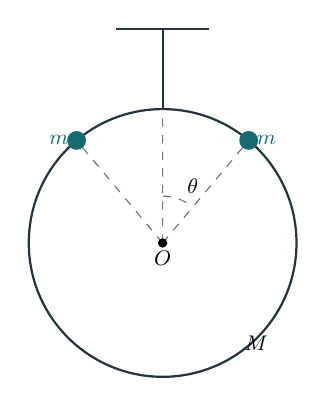
\begin{tikzpicture}[scale=.85,transform shape]

\draw[object] (0,0) circle (2);
\draw[object] (0,2)--(0,3.2);
\draw[object] (-.7,3.2)--(.7,3.2);
\fill[accent] (50:2) circle (4pt) node[right] {$m$};
\fill[accent] (130:2) circle (4pt) node[left] {$m$};
\draw[guide] (0,0)--(50:2) (0,0)--(130:2) (0,0)--(0,2);
\draw[guide] (0,.7) arc[start angle=90,end angle=50,radius=.7];
\node at (.45,.85) {$\theta$};
\fill (0,0) circle (2pt) node[below] {$O$};
\node at (1.4,-1.5) {$M$};

\end{tikzpicture}
\figcaption{图综五.3\quad 两珠穿环形成双向约束，悬绳只能提供向上拉力。}
\end{minipage}\end{center}

\par\vspace{5mm}\noindent{\small\color{muted}作答区}\par\vspace{3mm}\noindent\textcolor{rulegray}{\rule{\linewidth}{0.3pt}}\par\vspace{12mm}\noindent\textcolor{rulegray}{\rule{\linewidth}{0.3pt}}

\clearpage

\pdfbookmark[2]{第 4 题 一维气体绝热压缩的微观推导}{q4}

\section*{第 4 题\quad 一维气体绝热压缩的微观推导}\label{q:4}


柱形容器内有大量质量相同的小球，只沿容器长度方向往返运动，小球看作质点，彼此及与端面均作弹性正碰。速率和方向杂乱，以平均动能定义“温度”
\[
\overline\varepsilon=\frac12k_{\rm B}T.
\]
一端装有平面弹性活塞，沿容器长度方向缓慢向内推进。容器截面积固定，忽略重力和各种阻力，过程无热量交换。

从与移动活塞的碰撞出发，导出$T$与容积$V$的关系；说明相同质量小球间碰撞的作用，并用热容比及热力学第一定律分别推导同一关系。讨论范围是准静态压缩极限。


\begin{center}\begin{minipage}{.98\linewidth}\centering
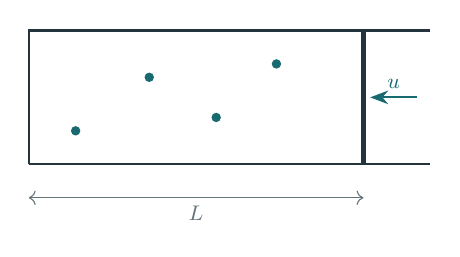
\begin{tikzpicture}[scale=.85,transform shape]

\draw[object] (0,0)--(0,2)--(6,2) (0,0)--(6,0);
\draw[object,line width=2pt] (5,0)--(5,2);
\foreach \x/\y in {.7/.5,1.8/1.3,2.8/.7,3.7/1.5}{\fill[accent] (\x,\y) circle (2pt);}
\draw[motion] (5.8,1)--(5.1,1) node[midway,above] {$u$};
\draw[axis,<->] (0,-.5)--(5,-.5) node[midway,below] {$L$};

\end{tikzpicture}
\figcaption{图综五.4\quad 一维质点只沿柱轴运动，活塞向内缓慢推进，截面积保持不变。}
\end{minipage}\end{center}

\par\vspace{5mm}\noindent{\small\color{muted}作答区}\par\vspace{3mm}\noindent\textcolor{rulegray}{\rule{\linewidth}{0.3pt}}\par\vspace{12mm}\noindent\textcolor{rulegray}{\rule{\linewidth}{0.3pt}}

\clearpage

\pdfbookmark[2]{第 5 题 直流导线中的电磁能流与焦耳热}{q5}

\section*{第 5 题\quad 直流导线中的电磁能流与焦耳热}\label{q:5}


一根无限长、圆截面的均匀直导线，半径为$R$，电导率为$\sigma$，通有沿轴向$+z$的恒定电流$I$。电流密度在截面上均匀。

（1）指出导线内坡印廷矢量（能流密度）的方向，并求随径向距离$r$的分布。（2）计算单位时间经长$l$的一段导线表面流入的能量。（3）证明它等于这段导线的焦耳热功率，并说明局部能量守恒。采用$\boldsymbol S=\boldsymbol E\times\boldsymbol H$。


\begin{center}\begin{minipage}{.98\linewidth}\centering
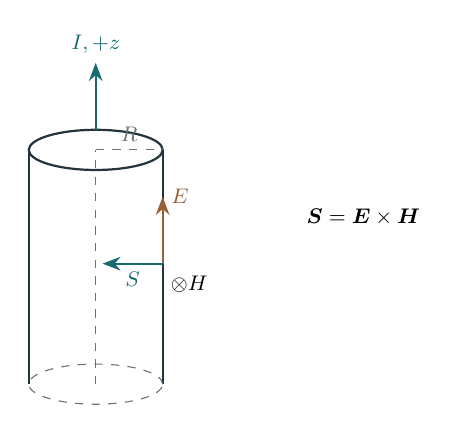
\begin{tikzpicture}[scale=.85,transform shape]

\draw[object] (-1,0)--(-1,3.5) (1,0)--(1,3.5);
\draw[object] (0,3.5) ellipse (1 and .3);
\draw[guide] (0,0) ellipse (1 and .3);
\draw[motion] (0,3.8)--(0,4.8) node[above] {$I,+z$};
\draw[guide] (0,0)--(0,3.5);
\draw[guide] (0,3.5)--(1,3.5) node[midway,above] {$R$};

\draw[force] (1,1.8)--(1,2.8) node[right] {$E$};
\node[right] at (1,1.5) {$\otimes H$};
\draw[motion] (1,1.8)--(.1,1.8) node[midway,below] {$S$};
\node at (4,2.5) {$\boldsymbol S=\boldsymbol E\times\boldsymbol H$};

\end{tikzpicture}
\figcaption{图综五.5\quad 电流沿轴向，电场轴向、磁场环向，能流从侧面径向流入。}
\end{minipage}\end{center}

\par\vspace{5mm}\noindent{\small\color{muted}作答区}\par\vspace{3mm}\noindent\textcolor{rulegray}{\rule{\linewidth}{0.3pt}}\par\vspace{12mm}\noindent\textcolor{rulegray}{\rule{\linewidth}{0.3pt}}

\clearpage

\pdfbookmark[2]{第 6 题 “王”字透光孔的夫琅禾费衍射}{q6}

\section*{第 6 题\quad “王”字透光孔的夫琅禾费衍射}\label{q:6}


均匀单色平面光以波长$\lambda$正入射一块不透明屏，屏上开有图示“王”字透光孔。孔由三个宽$3a$、高$a$的水平矩孔，以及连接它们的两个$a\times a$方孔拼成；各块只共边、不重叠。三个水平矩孔中心为$(0,0),(0,\pm2a)$，两个方孔中心为$(0,\pm a)$。

在透镜后焦面观察夫琅禾费衍射。透镜焦距为$f$，焦面横、纵坐标为$X,Y$，孔面为$x,y$，取方向余弦$q_x\simeq X/f,q_y\simeq Y/f$。导出远场复振幅和归一化光强，画出主要明暗结构；说明矩孔平移的相位如何进入叠加，并用轴向截面说明中央亮区的宽窄。用$\operatorname{sinc}z=\sin z/z$，$\operatorname{sinc}0=1$。


\begin{center}\begin{minipage}{.98\linewidth}\centering
\begin{tikzpicture}[scale=.85,transform shape]
\fill[accent!12] (-1.5,-0.5) rectangle (1.5,0.5);\draw[object] (-1.5,-0.5) rectangle (1.5,0.5);
\fill[accent!12] (-1.5,1.5) rectangle (1.5,2.5);\draw[object] (-1.5,1.5) rectangle (1.5,2.5);
\fill[accent!12] (-1.5,-2.5) rectangle (1.5,-1.5);\draw[object] (-1.5,-2.5) rectangle (1.5,-1.5);
\fill[warm!15] (-.5,0.5) rectangle (.5,1.5);\draw[object] (-.5,0.5) rectangle (.5,1.5);
\fill[warm!15] (-.5,-1.5) rectangle (.5,-0.5);\draw[object] (-.5,-1.5) rectangle (.5,-0.5);
\draw[axis] (-2.4,0)--(2.6,0) node[right] {$x$};
\draw[axis] (0,-3)--(0,3.2) node[above] {$y$};
\draw[axis,<->] (-2.8,-2.5)--(-2.8,2.5) node[midway,left] {$5a$};
\draw[axis,<->] (-1.5,-3.4)--(1.5,-3.4) node[midway,below] {$3a$};
\begin{scope}[xshift=7cm]
\draw[axis] (-1.8,0)--(2,0) node[right] {$X$};
\draw[axis] (0,-2)--(0,2.2) node[above] {$Y$};
\node at (0,-3) {后焦面：孔场的傅里叶分布};
\end{scope}

\end{tikzpicture}
\figcaption{图综五.6\quad 孔由五块互不重叠的矩孔拼成，孔面与焦面坐标方向对应。}
\end{minipage}\end{center}

\par\vspace{5mm}\noindent{\small\color{muted}作答区}\par\vspace{3mm}\noindent\textcolor{rulegray}{\rule{\linewidth}{0.3pt}}\par\vspace{12mm}\noindent\textcolor{rulegray}{\rule{\linewidth}{0.3pt}}

\end{document}
